\section{Simulating Longer Propagation Distances}
  \label{sec:simultons_long}

    Thus far we have considered the behaviour of the atomic medium as addressed
    by the \textsc{cw} probe and disturbed by the strong pulse over the
    propagation distance of the thin cell. The restricted propagation distance
    is a limit of the current experimental setup, but in our numerical
    simulations we are not subject to the same constraint. We may extend the
    propagation medium arbitrarily far to observe what happens to both the atoms
    and the propagating fields. This will complete our analysis of the observed
    signal response, and also allow us to make predictions for future laboratory
    studies.

  \subsection{Propagation in the Coupling Pulse Scheme}

    We will first consider some demonstration cases, before looking at the
    specific parameters for the experimental system. We know from the study of
    two- and three-level media in chapter \ref{chp:nonlinear} that a key
    property in the propagation of short pulses in nonlinear systems is the
    pulse area $\theta$ defined in equation \ref{eqn:pulse_area}. Thus we'll
    design simulations with fixed input pulse areas, rather than specifying the
    peak intensities as we have done so far. Of course, for a given Gaussian
    pulse width, these definitions are interchangeable.

    We will for now neglect the motional and hyperfine pumping effects we added
    to the model in section \ref{sec:simultons_theory}, as we seek to gain
    physical insight into the specific effects of propagation.

    \begin{figure}[h]
    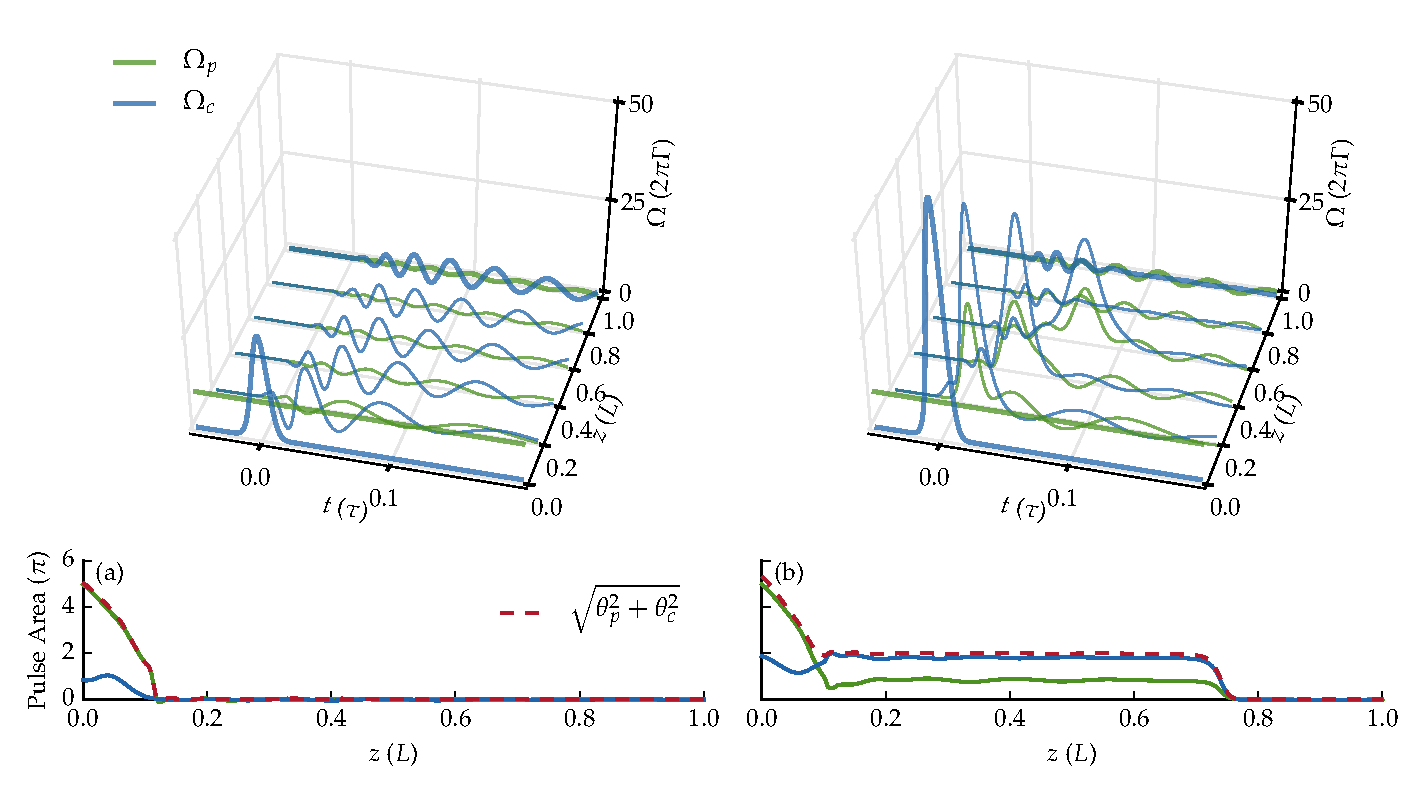
\includegraphics[width=\linewidth]
      {figs/06_simultons/mb_vee_sit_plot_08pi_18pi_fig1.pdf}
    \caption{
    Propagation of (a) $0.8 \pi$ and (b) $1.8 \pi$ coupling pulses (blue)
    through a medium addressed by a $\unit[10]{\Gamma}$ \textsc{cw} probe
    (green), showing (top) profiles of the real part of the complex Rabi
    frequencies $\Omega(z, \tau)$ and (bottom) pulse areas $\theta(z)$.
    }
    \label{fig:pulse_cw_08pi_18pi}
    \end{figure}

    In figure \ref{fig:pulse_cw_08pi_18pi} we present numerical results for the
    \textsc{cw} probe, coupling pulse scheme in a medium with absorption
    coefficients set at $N g_{01} = N g_{02} = \unit[2\pi~10^3]{\Gamma/L}$. This
    is an order of magnitude larger than those representing the thin cell
    experiments, and therefore represents a longer distance of propagation. The
    coupling input pulses are Gaussians of width $\tau_w = $
    \unit[0.01]{$\tau_\Gamma$} and have pulse areas of (a) $0.8 \pi$
    (corresponding to a peak $\Omega_c = \unit[2\pi~28]{\Gamma}$) and (b) $1.8
    \pi$ (a peak $\Omega_c = \unit[2\pi~62]{\Gamma}$). In both cases the
    \textsc{cw} probe is strong with Rabi frequency $\Omega_p =
    \unit[2\pi~10]{\Gamma}$.

    In figure \ref{fig:pulse_cw_08pi_18pi}(a) we see that for the $0.8 \pi$ pulse both
    the \textsc{cw} probe and the coupling pulse are absorbed close to the front
    of the medium, with the pulse area dissipated by around $z = $
    \unit[$0.1$]{$L$}. From then on the only remnant of the fields is the fast
    ringing.

    In figure \ref{fig:pulse_cw_08pi_18pi}(b) we see that for the $1.8 \pi$
    pulse, the large coupling pulse kicks up a pulse from the \textsc{cw} field,
    consistent with our analysis of a period of reduced absorption. Of interest
    in this long distance simulation is that the resultant probe pulse is able
    to form its own steady-state soliton, as described in the study of matched
    pulses in chapter \ref{chp:nonlinear}. Rather than dissipating entirely, the
    probe pulse area $\theta_p$ (bottom, green) is held abruptly at around $z =
    $ \unit[$0.1$]{$L$} to a value of around $1 \pi$. The simultaneous
    propagating pulses first steepen toward the sech shape, but then broaden and
    slow due to the spontaneous decay. We see the large area of the \textsc{cw}
    probe decreases but doesn't disappear, and the combined pulse area $\theta =
    \sqrt{\theta_p^2 + \theta_c^2}$ (bottom, red dashed) finds its steady state
    at $2 \pi$. The pulses do not reach the end of the medium in the duration of
    the simulation, propagating a distance of $z = $ \unit[$0.7$]{$L$}.

    We may ask: what does it means to define a pulse area for an input
    \textsc{cw} field? For our purposes, we may take it to be arbitrarily large.
    Numerically, we integrate the Rabi frequency envelope over the duration of
    the simulation. The key point is that in the case that the combined pulse
    area is large enough to support simultaneous propagation, this arbitrarily
    large pulse area does not dissipate but is held.

    What happens for stronger pulses? In figures \ref{fig:pulse_cw_4pi_cmap} and
    \ref{fig:pulse_cw_6pi_cmap} we present results for larger-area pulses input
    on the same medium with the same \textsc{cw} probe field of $\Omega_p =
    \unit[10]{\Gamma}$. The coupling input pulses are again Gaussians of width
    $\tau_w = $ \unit[0.01]{$\tau_\Gamma$}.

    \begin{figure}%[h]
    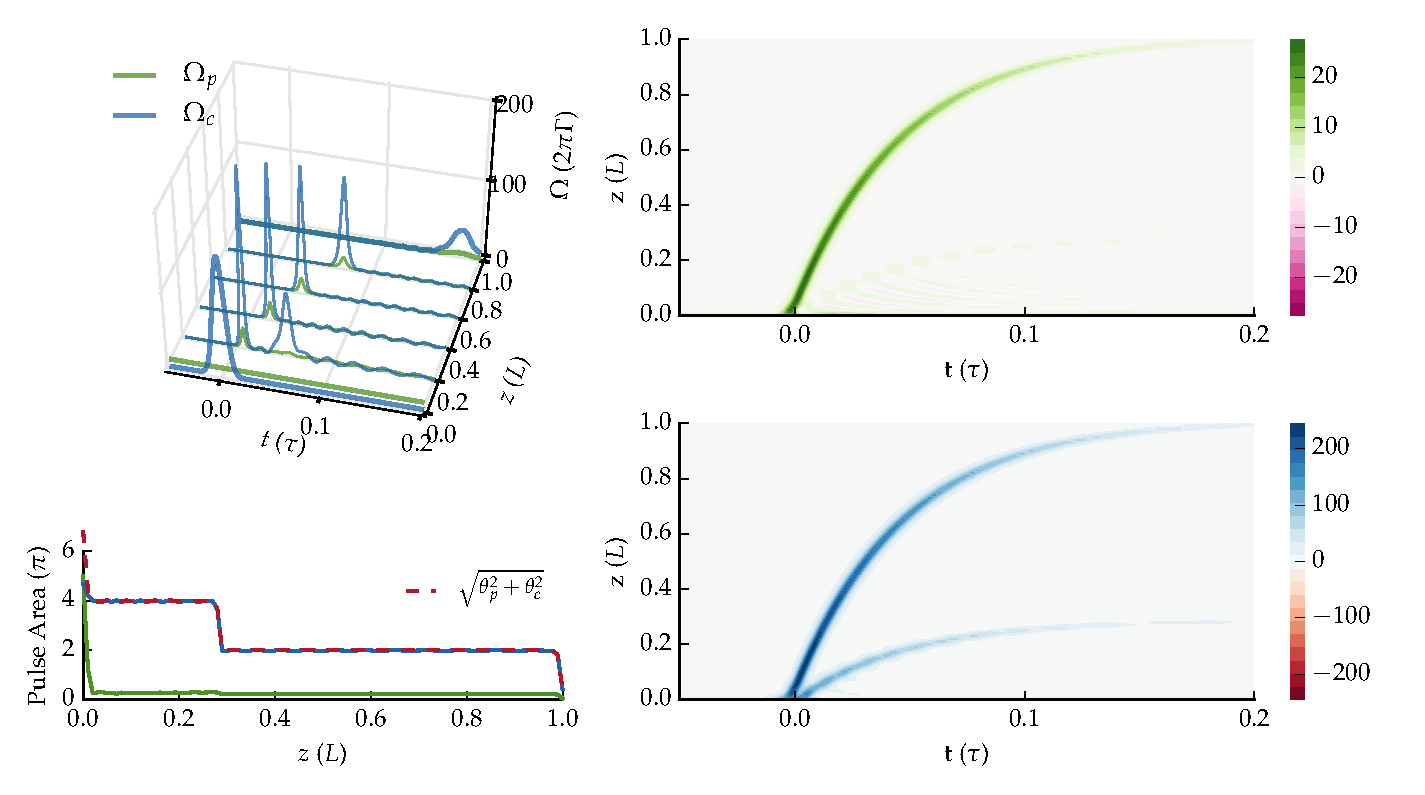
\includegraphics[width=\linewidth]
      {figs/06_simultons/mb_vee_sit_plot_45pi_Ng1e4_fig1.pdf}
    \caption{
    Propagation of a Gaussian $4.5 \pi$ input coupling pulse with width
    \unit[$0.01$]{$\tau_\Gamma$} through a V-type medium addressed by a
    $\unit[10]{\Gamma}$ \textsc{cw} probe. (Top left) Propagation profile of the
    probe (green) and coupling (blue) fields. (Bottom left) Pulse areas of the
    fields and the total area (red dashed). (Right) Colourmaps of the real part
    of the complex Rabi frequencies $\Omega_{p}$ and $\Omega_{c}$.
    }
    \label{fig:pulse_cw_4pi_cmap}
    \end{figure}

    In figure \ref{fig:pulse_cw_4pi_cmap}, for the $4.5 \pi$ pulse, we see the
    coupling pulse break apart as we've seen previously. Again we see that the
    pulse kicks up a simultaneous pulse in the probe field as the absorption is
    initially reduced, which allows a small pulse area to move through, and this
    is carried on by the first resultant $2 \pi$ pulse.

    We may understand the reason that only one pulse propagates in the probe
    field by considering the evolution of the off-diagonal matrix elements we
    presented in figure \ref{fig:sim_0703_temp_210C_build0_coh}. For every two
    oscillations in $\rho_{02}$, the system evolves through one oscillation in
    $\rho_{01}$. This oscillation forms the probe component of a pulse that
    matches with the first coupling pulse and propagates as a simulton.

    \begin{figure}%[h]
    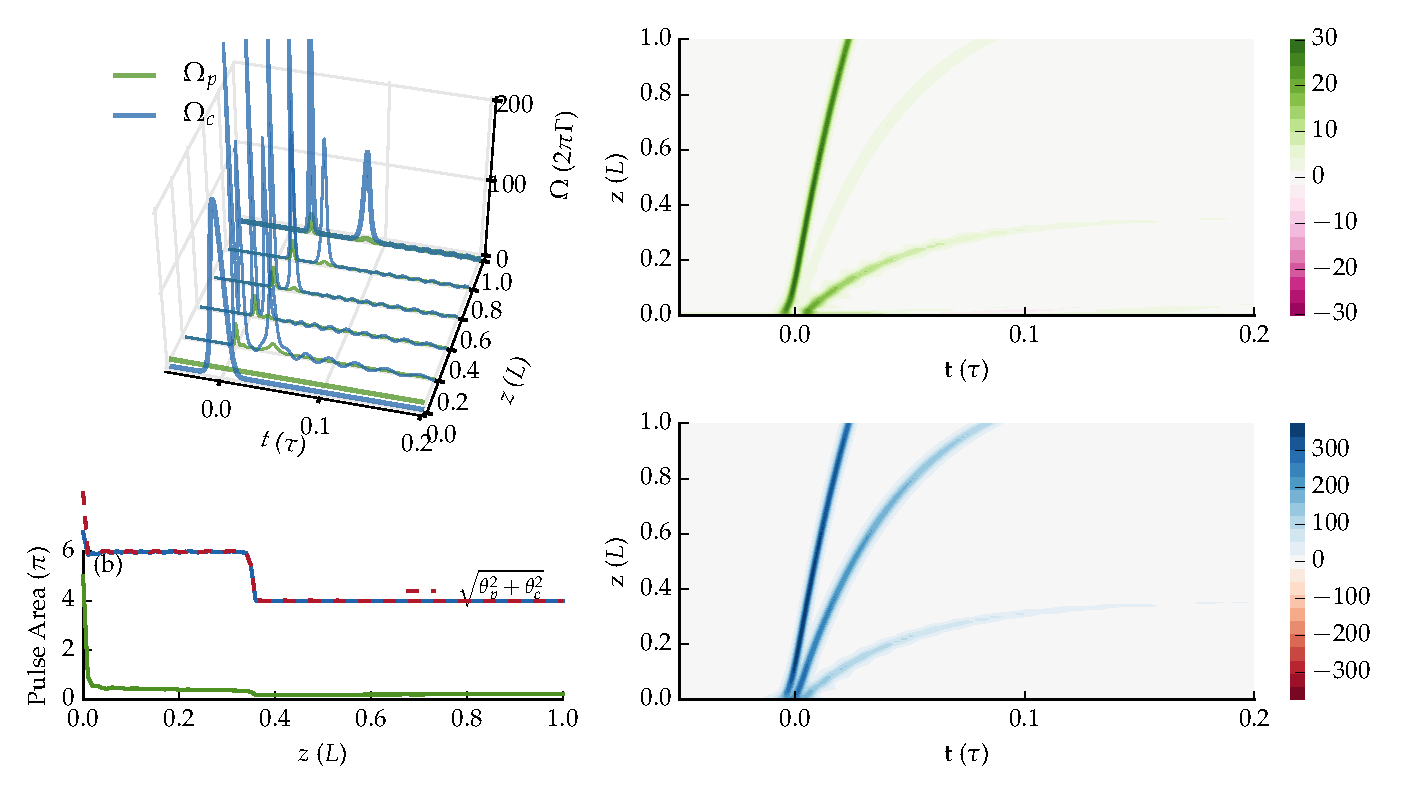
\includegraphics[width=\linewidth]{figs/06_simultons/mb_vee_sit_plot_65pi_Ng1e4_fig1.pdf}
    \caption{
    Propagation of a Gaussian $6.5 \pi$ input coupling pulse with width
    \unit[$0.01$]{$\tau_\Gamma$} through the V-type medium addressed by a
    $\unit[10]{\Gamma}$ \textsc{cw} probe. (Top left) Propagation profile of the
    probe (green) and coupling (blue) fields. (Bottom left) Pulse areas of the
    fields and the total area (red dashed). (Right) Colourmaps of the real part
    of the complex Rabi frequencies $\Omega_{p}$ and $\Omega_{c}$.
    }
    \label{fig:pulse_cw_6pi_cmap}
    \end{figure}

    In figure \ref{fig:pulse_cw_6pi_cmap}, for the $6.5 \pi$ pulse, we see that
    the coupling pulse breaks into three resultant pulses as we'd expect and the
    kicked up pulse area in the probe field is carried mostly by the first and
    third resultant $2 \pi$ pulses.

    [TODO: Clarify the argument.]

    These demonstrative simulations provide an interesting result: a portion of
    the \textsc{cw} probe field is in fact picked up by the strong pulse and
    carried along as a simultaneous pulse with the same width, at the same
    velocity, and capable of propagating over long distances.

  \subsection{Comparison with Experimental Data}

    The discovery that a strong coupling pulse has the effect of causing a long-
    distance propagating soliton in the \textsc{cw} probe leads us to consider
    the experimental results from the thin cell, using the parameters of section
    \ref{sec:simultons_experiment}, but imagining that the cell is longer.
    Recall that in the case of transitions on the the rubidium \textsc{d1} and
    \textsc{d2} lines we have distinct values for $g_{01}$ and $g_{02}$, as they
    are proportional to the square of the respective dipole moments, $d_{0j}^2$.
    This may affect the ability of the pulses to match and propagate.

    \begin{figure}[h]
      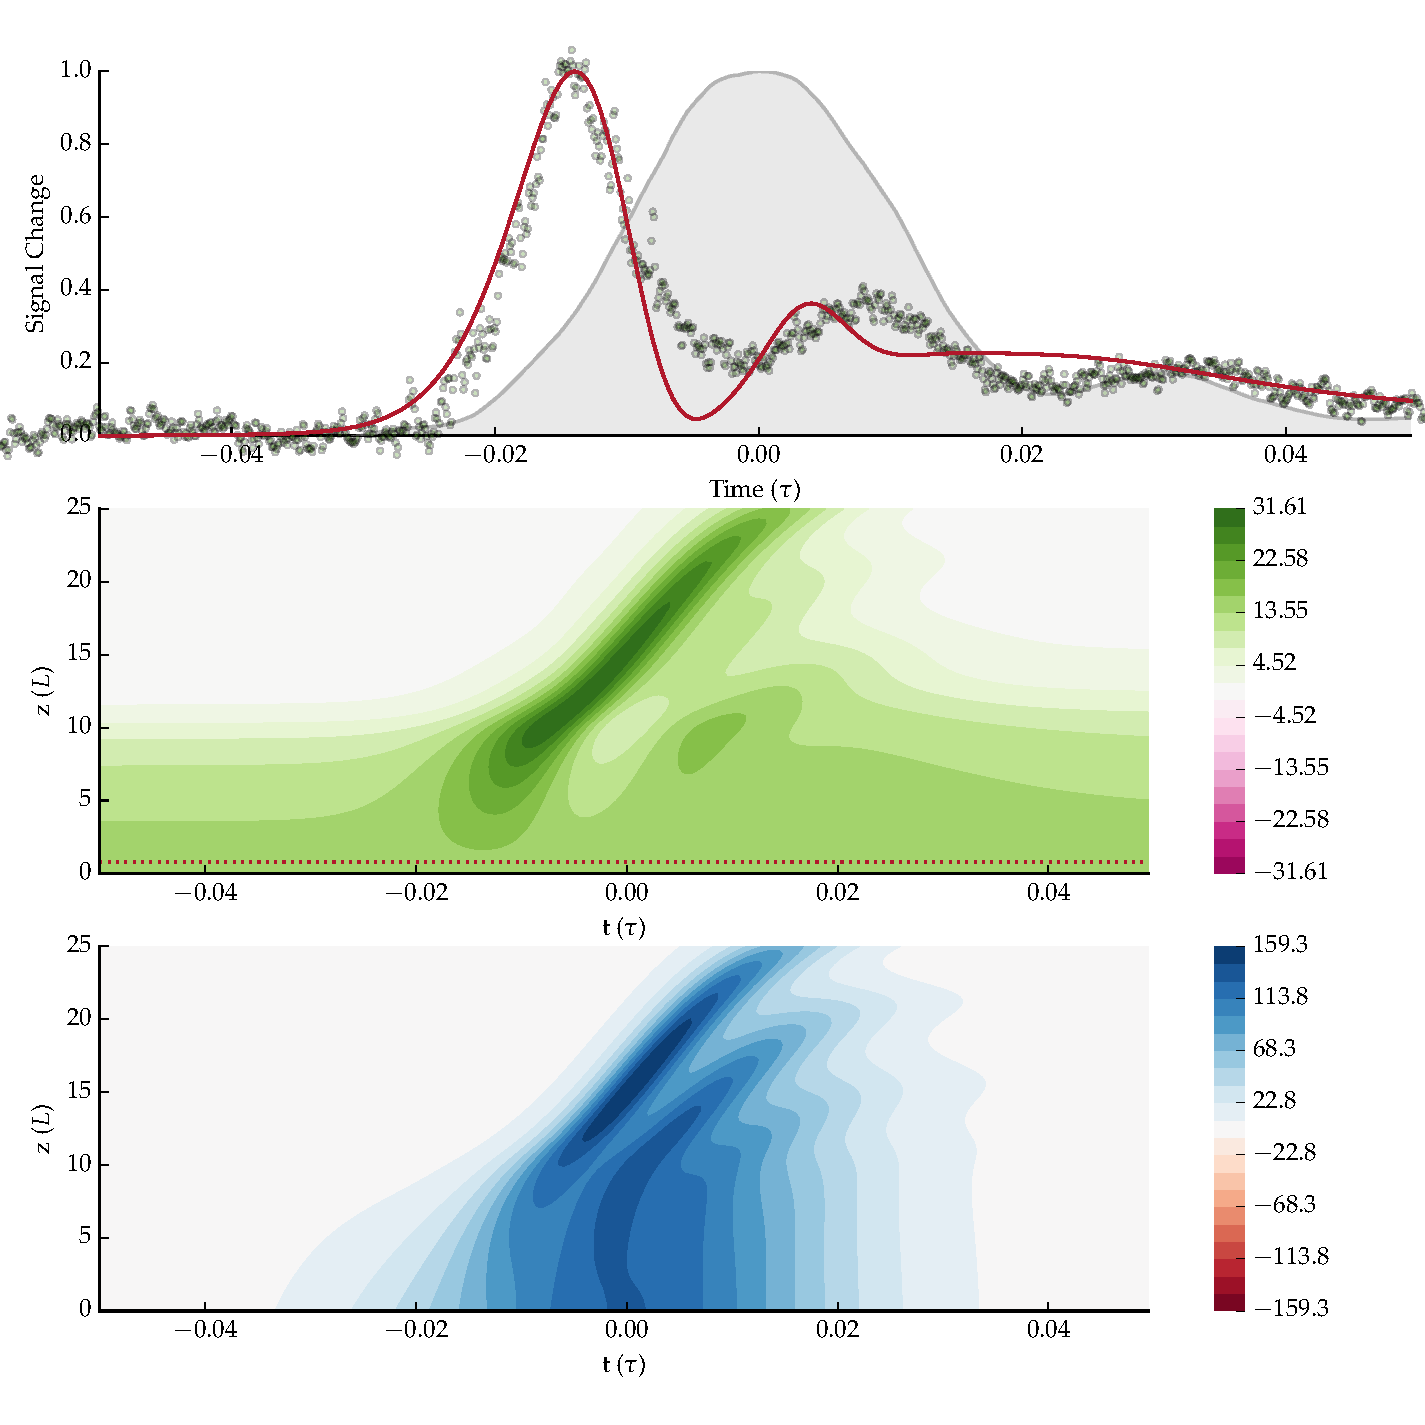
\includegraphics[width=\linewidth]
        {figs/06_simultons/mb_vee2g_15c_130p_0330t_230C_sb50_120vel010_10_050um_fig1.pdf}
      \caption{
      (Top) Comparison of numerical results (red) with experimental data (blue
      circles) for the normalised transmitted probe signal. The measured coupling
      pulse signal (grey filled area) has a width $\tau_w = $ \unit[$0.80$]{ns} $
      \equiv $ \unit[$0.029$]{$\Gamma_\tau$} in each case. The temperature is
      \unit[$230$]{\textdegree C}. (Middle) Colour map of the real part of the
      complex Rabi frequency for the probe field. The red dotted line marks $z =
      1L$. (Bottom) Colour map of the real part of the complex Rabi frequency for
      the coupling pulse.
      } 
      \label{fig:exp_result_single} 
    \end{figure}

    In figure \ref{fig:exp_result_single} we present again the comparison of
    numerical result and experimental data shown in figure
    \ref{fig:sim_data_0703_temp_210C}. In the experiment the temperature $T =
    \unit[230]{\textrm{\textdegree C}}$, and the peak pulse power is
    \unit[$85$]{mW}, and the same parameters are simulated. We again present the
    real part of $\Omega_p$ and $\Omega_c$ but continue the simulation over a
    longer distance, imagining that the cell is much longer at \unit[$50$]{$\mu
    m$} $ \equiv$ \unit[$25$]{$L$}. This will allow us to predict the long-
    distance behaviour.

    The coupling pulse has a large pulse area $\theta_c = 9.1 \pi$, and so over
    the longer distance we start to see the same pulse break-up we saw in
    figures \ref{fig:pulse_cw_4pi_cmap} and \ref{fig:pulse_cw_6pi_cmap}. Again
    it is the earliest resultant pulse which carries along a pulse in the probe
    field, rising before the centre of the pulse at $t = 0$. The later resultant
    pulses in the coupling field are unable to propagate far into the medium due
    to the dephasing effect of collision broadening.

    The simulated result of the field propagation over longer-distances thus
    gives us an understanding of the mechanism behind the observed transmission
    profiles in the probe field when the system is disturbed by the strong
    coupling pulse. We see that \textit{it is the formation of this nascent
    soliton} in the probe field which causes the steep early in the experimental
    signal as the probe field is shaped towards a sech-shaped soliton.

    It also explains why the peak intensity increases with temperature and
    number density as observed in figure \ref{fig:exp_result_temp_dep}, as we
    are in the nascent stage when the pulse is being shaped. We expect it to
    saturate as the sech-shape reaches its steady state, and this may be what we
    see in figure \ref{fig:data_0703_temp_all} at the highest temperature
    investigated of $T = \unit[290]{\textrm{\textdegree C}}$.

  \subsection{Hyperfine Structure \& Degeneracy}

    A complete account of the electronic energy level structure of rubidium
    would include fine and hyperfine structure, as considered for the model in
    chapter \ref{chp:twophoton}. Approximating the rubidium vapour as a three-
    or four-level atomic medium appears to be justified here on the basis that
    the simulated transmission profiles provide a good qualitative fit to the
    data along with physical insight into the underlying coherent mechanism.

    The discovery, however, that pulse propagation effects are significant means
    that the physical structure of the atomic energy levels requires further
    consideration. This is clear if we consider the pulse area, introduced in
    chapter \ref{chp:nonlinear}, which is given by
    \begin{equation}
      \Theta(z) = \int^\infty_{-\infty} \Omega(z,t) \dd t
                = \frac{d}{\hbar} \int^\infty_{-\infty} \mathcal{E}(z,t) \dd t.
    \end{equation}
    This quantity is well-defined only if the atomic levels coupled have a
    uniquely specified dipole moment $d$. We understand that the physical system
    in fact has this deeper hyperfine structure due to coupling of the
    electron's orbital angular momentum $L$, spin $S$ and the nuclear spin $I$,
    as shown in figure \ref{fig:rb85_levels}. An additional concern is that, in
    the absence of an applied magnetic field, the $2F + 1$ sublevels of these
    hyperfine $F$ levels are spatially degenerate such that there is no
    straightforward way for these $m_F$ states to be addressed separately.

    The couplings between these degenerate sublevels will then have different
    dipole matrix elements $\Bra{F m_F} e \mathbf{r} \Ket{F' m'_F}$ and
    therefore different Rabi frequencies $\Omega$,  and this can be expected to
    suppress the formation of coherent optical solitons.

    However, in the case of the experimental study of this chapter, the
    shortness of pulse duration  is such that its spectral width is on the order
    of \unit[$\sim 2\pi~1$]{GHz}. The hyperfine manifolds of the
    $5^2\mathrm{P}_{\nicefrac{1}{2}}$ and $5^2\mathrm{P}_{\nicefrac{3}{2}}$
    levels are spread over an energy range on the order of \unit[$\sim
    2\pi~100$]{MHz}, so the pulse interacts with the full manifold of excited
    state hyperfine levels $J \rightarrow J'$, and this excited hyperfine
    structure is not accessible.

    [TODO: RP says the following is only generally true in the case where J = 0
    [or 1/2. Make reference to personal communication from RP.]

    Taking just a single $J \rightarrow J'$ transition for now, the effective
    dipole moment for a particular ground state sublevel $\Ket{F m_F}$ is then
    found by summing the coupling to all of these excited state sublevels.  In
    the case of linearly-polarised light, coupling levels such that the angular
    momentum difference $q = m_F' - m_F = 0$, we have\cite{Steck2001}
    \begin{equation}\label{eqn:hf_factor}
      \sum_{F'} (2 F' + 1)(2 J + 1) 
        \begin{Bmatrix}
          J & J' & 1 \\[8pt]
          F' & F & I
        \end{Bmatrix}^2
        \lvert \langle F~m_F \vert F'~1~m_F~0 \rangle \rvert^2 = \frac{1}{3}
    \end{equation}
    independent of the particular values of $F$ and $F'$ such that the effective dipole moment is given by
    \begin{equation}\label{eqn:dipole_symm_factor}
      d = 
        \sqrt{\frac{1}{3}} \langle J || e \mathbf{r} || J' \rangle.
    \end{equation}
    for \textit{every} sublevel $\Ket{F m_F}$, where $\langle J || e \mathbf{r}
    || J' \rangle$ is the reduced dipole operator for the fine structure
    transition, which is known experimentally from the natural linewidth.

    This factor of $\sqrt{\nicefrac{1}{3}}$ can be understood as due to
    spherical symmetry, by considering that the linearly polarised light will
    interact with only one of the spherical components of the dipole operator.

    Then what about the orthogonal, linearly-polarised beam? As we have defined
    the first transition to be the $\pi$ ($q = 0$) transition, the orthogonal
    beam is defined by a polarisation vector $\left( \sigma_+ + \sigma_- \right)
    / \sqrt{2}$, a symmetric combination of photons either adding or subtracting
    a quantum of angular momentum to the atom. By making a summation as in
    equation (\ref{eqn:hf_factor}) for the $q = 1, -1$ transitions, we find the
    same $\nicefrac{1}{\sqrt{3}}$ factor, which we would expect again by
    considering the symmetry of the system.

    The result is then for the system to respond as if there were indeed a
    unique dipole moment, but one which must take into account the symmetry
    factor in equation (\ref{eqn:dipole_symm_factor}) and we are justified in
    applying the simple three-level model.

  \subsection{Weak Probe Fields}

    Thus far we have considered examples of propagation in the \textsc{cw} probe
    scheme in which the field is strong. Such strong fields were required in the
    experiment in order to achieve good detection on the fast photon counter
    employed. Theoretically, however, we are inclined to consider weak pulses as
    they may be useful in applications such as quantum information processing
    and storage.

    As described in chapter \ref{chp:nonlinear}, the pulse area theorem in the
    case of three-level V-type systems applies not to the individual pulse
    areas, but to their sum in quadrature. This suggests that if the coupling
    pulse applied on the adjacent transition is strong, we may be able to
    consider the scheme for propagation of weak probe through a medium to which
    it would normally be opaque.

    \begin{figure}[]
      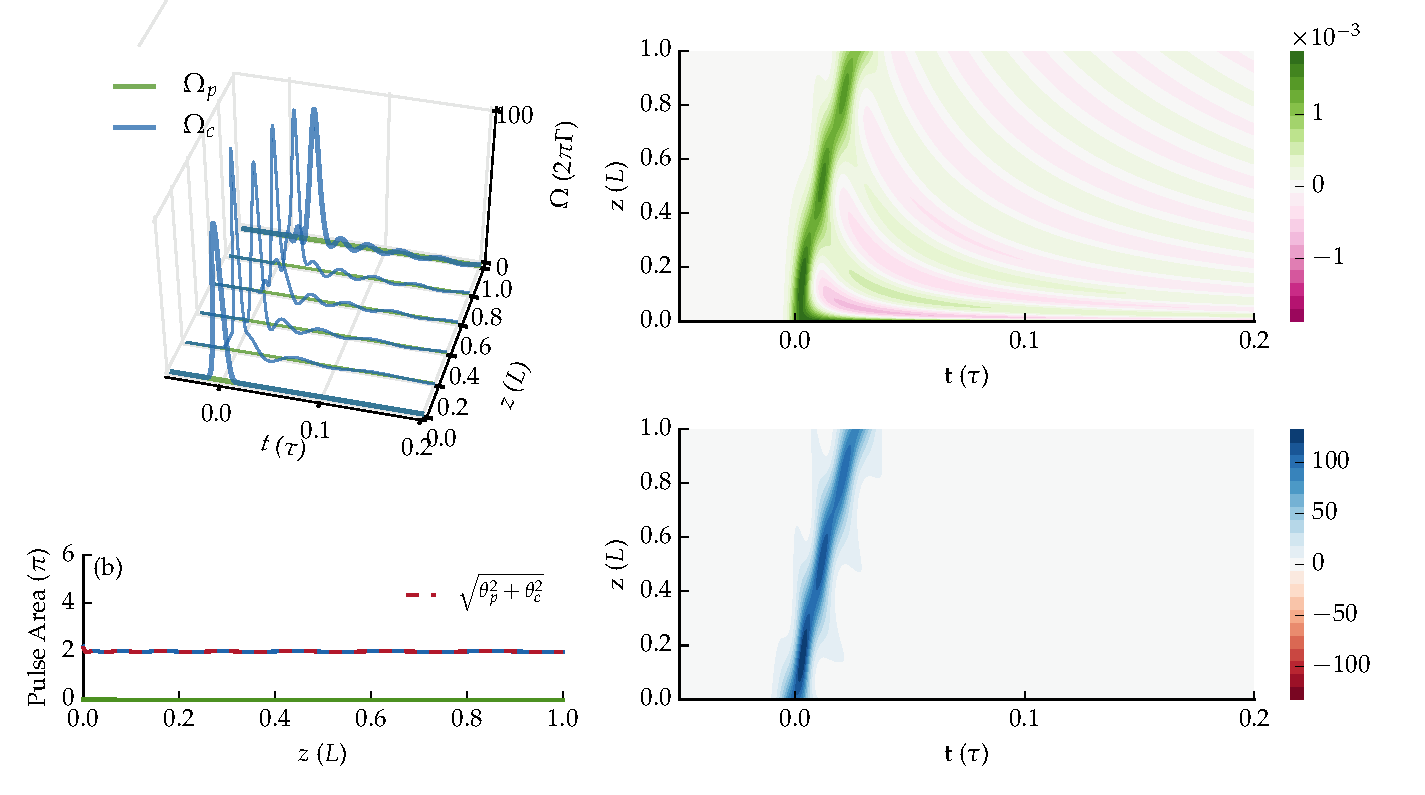
\includegraphics[width=\linewidth]
        {figs/06_simultons/mb_vee_wpsit_plot_001c_22pip_Ng1e3_fig1.pdf}
      \caption{
      Propagation of a $2.2\pi$ Gaussian input coupling pulse with width
      \unit[0.01]{$\tau$} through the V-type medium addressed by a weak
      $\Omega_p~=$~\unit[$0.001$]{$\Gamma$} \textsc{cw} probe field. The number
      density is such that $Ng = \unit[2\pi~10^3]{\Gamma/L}$. (Top left)
      Propagation profile of the probe (green) and coupling (blue) fields.
      (Bottom left) Pulse areas of the fields and the total area (red dashed).
      (Right) Colourmaps of the real part of the complex Rabi frequencies
      $\Omega_p$ and $\Omega_c$.
      } 
      \label{fig:wp_propagation} 
    \end{figure}

    In figure \ref{fig:wp_propagation} we present numerical results which
    indicate that this is indeed the case. The input Gaussian has a pulse area
    of $2.2\pi$, while the \textsc{cw} probe field has a Rabi frequency of only
    \unit[$0.001$]{$\Gamma$}.

    Before the pulse, the probe field is absorbed immediately by the medium. We
    see that as for the strong probe field, the coupling pulse allows
    transmission of the probe field. We observe that this weak probe, despite
    being weak enough to excite only a tiny fraction of the atomic population to
    the $\rho_{11}$ state, is able to propagate simultaneously with the coupling
    pulse just as the strong probe was.  The three-level pulse area is nearly
    all in the coupling field, but the induced pulse in the probe field is not
    attenuated as it would be were the coupling field not present. Some high-
    frequency ringing is seen in the probe field.
    \begin{figure}[]
      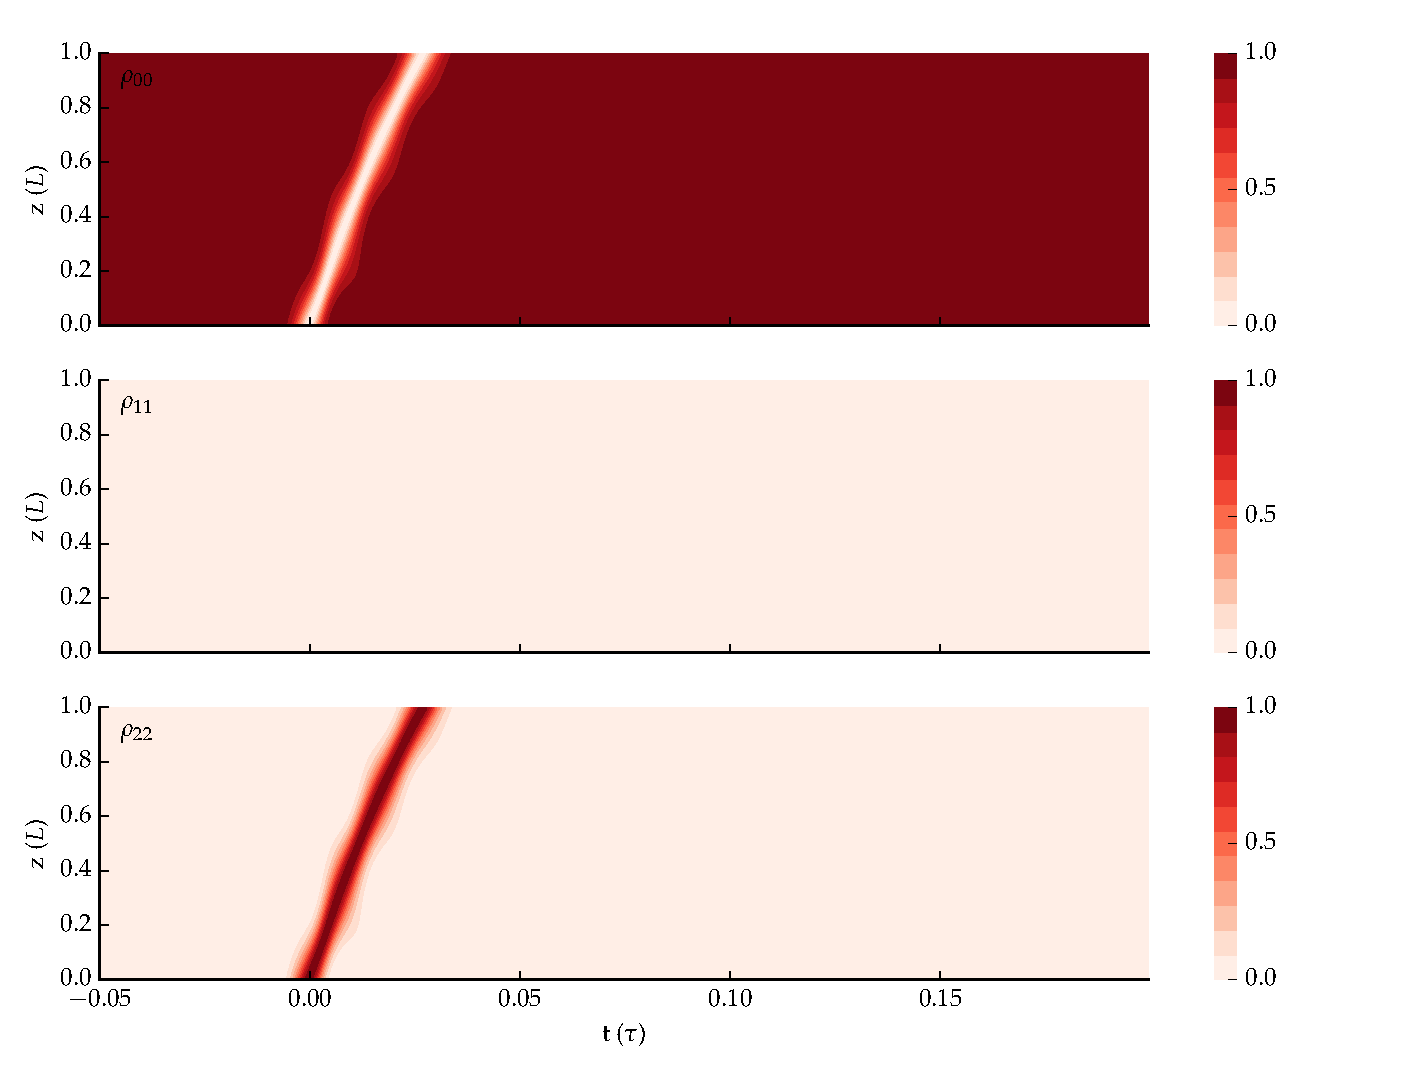
\includegraphics[width=\linewidth]
        {figs/06_simultons/mb_vee_wpsit_plot_001c_22pip_Ng1e3_fig2.pdf}
      \caption{
      Populations of the ground state (top) $\rho_{00}$ and excited states
      $\rho_{11}$ (middle) and $\rho_{22}$ (bottom) over $z$ and $t$ during the
      \unit[0.01]{$\tau$} through the V-type medium addressed by a weak
      $\Omega_p~=$~\unit[$0.001$]{$\Gamma$} \textsc{cw} probe field, as shown in
      figure \ref{fig:wp_propagation}.
      } 
      \label{fig:wp_pops} 
    \end{figure}

    Figure \ref{fig:wp_pops} shows the populations of the atomic states. We see
    propagation of a $2.2\pi$ Gaussian input coupling pulse with width that the
    propagation of the induced pulse in the probe field occurs despite
    negligible population transfer to the $\Ket{1}$ excited state. The
    population is nearly entirely transferred from the ground state $\Ket{0}$ to
    the $\Ket{2}$ excited state.

